\documentclass[conference]{IEEEtran}
\IEEEoverridecommandlockouts

% =========================================================================
% REQUIRED IEEE & TIKZ PACKAGES
% =========================================================================
\usepackage{cite}
\usepackage{amsmath,amssymb,amsfonts}
\usepackage{algorithmic}
\usepackage{graphicx}
\usepackage{textcomp}
\usepackage{xcolor}
\usepackage{booktabs}
\usepackage{multirow}
\usepackage{url}
\usepackage{microtype}
\usepackage{balance}
\usepackage{tikz}
\usetikzlibrary{shapes.geometric, arrows.meta, positioning, calc, shadows}

\hyphenation{op-ti-cal net-works semi-conduc-tor neu-ro-im-ag-ing pre-pro-cess-ing}

\begin{document}

% =========================================================================
% TITLE
% =========================================================================
\title{NeuroBehavior-ASD: Deep Learning-Based Autism Detection Using Brain Imaging Biomarkers and Behavioral Features with personalized support system\\
\thanks{*Note: Subtitles are not captured in Xplore and should not be used}
}

% =========================================================================
% AUTHORS & AFFILIATIONS (6 AUTHORS - EXACT MATCH)
% =========================================================================
\author{
\IEEEauthorblockN{1st Pavithra B}
\IEEEauthorblockA{\textit{Dept of CSE (DATA SCIENCE)} \\
\textit{Sai Vidya Institute of Technology}\\
Bangalore, India \\
pavithra.b@svividya.ac.in}
\and
\IEEEauthorblockN{2nd Dr Nagashree N}
\IEEEauthorblockA{\textit{Dept of CSE (DATA SCIENCE)} \\
\textit{Sai Vidya Institute of Technology}\\
Bangalore, India \\
nagashree.n@svividya.ac.in}
\and
\IEEEauthorblockN{3rd Shubhashree P}
\IEEEauthorblockA{\textit{Dept of CSE (DATA SCIENCE)} \\
\textit{Sai Vidya Institute of Technology}\\
Bangalore, India \\
shubhashreep.23ds@svividya.ac.in}
\vspace{0.2cm}
\and
\IEEEauthorblockN{4th Shriraksha M}
\IEEEauthorblockA{\textit{Dept of CSE (DATA SCIENCE)} \\
\textit{Sai Vidya Institute of Technology}\\
Bangalore, India \\
shriraksham.23ds@svividya.ac.in}
\and
\IEEEauthorblockN{5th Sushmitha A R}
\IEEEauthorblockA{\textit{Dept of CSE (DATA SCIENCE)} \\
\textit{Sai Vidya Institute of Technology}\\
Bangalore, India \\
sushmithaar.23ds@svividya.ac.in}
\and
\IEEEauthorblockN{6th Vanuja T V}
\IEEEauthorblockA{\textit{Dept of CSE (DATA SCIENCE)} \\
\textit{Sai Vidya Institute of Technology}\\
Bangalore, India \\
vanujatv.23ds@svividya.ac.in}
}

\maketitle

% =========================================================================
% ABSTRACT
% =========================================================================
\begin{abstract}
Autism Spectrum Disorder (ASD) is a neurodevelopmental condition that can affect communication, learning, and social. Early identification can help children access appropriate support. This paper presents NeuroBehavior-ASD, a web-based platform that combines brain MRI classification, behavioral screening, and healthcare resource discovery. The MRI component explores deep learning techniques using the ABIDE dataset, along with image enhancement and brain symmetry features. This work achieved 95.21\% accuracy and a ROC-AUC of 0.9814 on the test partition. The platform also includes a separate Indian Autism Screening Questionnaire (IASQ) module, report generation, and location-based healthcare recommendations. The system aims to support research and improve access to relevant services.
\end{abstract}

\begin{IEEEkeywords}
Autism Spectrum Disorder, Deep Learning, Magnetic Resonance Imaging (MRI), Behavioral Analysis.
\end{IEEEkeywords}

% =========================================================================
% SECTION I: INTRODUCTION
% =========================================================================
\section{Introduction}
Autism Spectrum Disorder (ASD) is a neuro-developmental disorder that can cause differences in brain development, cognitive functioning and behaviour. An important research topic in this area is how early we can detect these differences. Current methods of identifying these differences are mostly based around observing behaviours, consulting professionals and using screening questionnaires. This can be a lengthy process requiring lots of specialist knowledge. Medical imaging and Artificial Intelligence have made huge developments in the last few years \cite{namitha2026}, meaning there are new opportunities to look at patterns in the brain and create computer based methods for ASD screening. This means there is a need for easily accessible, technology based solutions.

Brain Magnetic Resonance Imaging (MRI) has gained attention in autism research because it helps researchers study brain structure and patterns associated with ASD \cite{hasan2025}. Deep learning techniques offer a way to analyze these images and explore their usefulness in classifying ASD and control groups. In this project, MRI data covering the age range of 0 to 64 years are considered. However, differences in brain characteristics, image quality, and scanning sites can make classification challenging.

Another challenge is making MRI analysis accessible through a simple system. Medical images may be available in different formats, and some approaches require significant computing resources. In addition, MRI classification alone does not provide information about a person's everyday behavior or help families find suitable support services.

To address these challenges, this paper presents NeuroBehavior-ASD, a web-based platform that explores deep learning-based MRI classification using the ABIDE dataset. The system also provides a separate behavioral screening module based on the Indian Autism Screening Questionnaire (IASQ), along with report generation, assessment history, and location-based healthcare resource recommendations.

The main contributions of this project are:
\begin{itemize}
    \item \textbf{MRI classification:} Explore deep learning methods to classify ASD and control MRI images.
    \item \textbf{Image processing:} Investigate image enhancement and brain symmetry features.
    \item \textbf{Behavioral screening:} Provide an independent questionnaire-based screening module.
    \item \textbf{Report and support services:} Generate assessment reports and help users discover relevant healthcare resources based on location.
\end{itemize}

The platform is intended to provide an organised source of information on assessments plus help you find the right support. It is for research/information purposes only and should not be used as a clinical diagnosis or a substitute for professional assessment.

% =========================================================================
% SECTION II: RELATED WORK
% =========================================================================
\section{Related Work}

\subsection{Past Computer Methods for Autism}
With the release of public brain datasets such as ABIDE \cite{gkintoni2025}, researchers have looked to use machine learning techniques to detect autism \cite{rathod2026, mathkor2026}. These early techniques used software such as FreeSurfer to measure cortical thickness. However, this can take a long time (8--12 hours) per patient and the software often does not work if there are small shadows in the scan.

A Split and Merge U-Net approach is proposed for the automatic detection of autism using brain MRI images by focusing on segmentation of corpus callosum using deep learning techniques and ABIDE dataset \cite{nagashree2024}.

Researchers have since looked at using deep neural networks. Some have used resting state fMRI to look at connectivity in the brain, achieving around 70\% accuracy \cite{shankari2026, munoz2026}. Others have looked at using 3D neural networks with structural MRI \cite{polavarapu2026}. However, due to high memory requirements, the images had to be reduced in size, achieving around 65--72\% accuracy.

Recently, computer vision researchers discovered that models trained on everyday photos (like MobileNetV2 \cite{anyom2025}) can be adapted for medical images. Because MobileNetV2 is small and fast, it can detect edges, corners, and brain textures without needing large computers.

\subsection{Parent Questionnaires}
In clinics, doctors always start by asking parents questions about how their child behaves. In Western countries, the M-CHAT questionnaire is popular \cite{vignapiano2025}. The ISAA scale was developed by the government in India \cite{xu2025}. This has since been developed by medical researchers into a 10 item validated screening questionnaire called the Indian Autism Screening Questionnaire (IASQ) \cite{wakelin2026}. A score of 2 or more on the IASQ has over 80\% accuracy in identifying children who need specialist help.

\subsection{Responsible Medical AI}
Medical AI tools should never try to replace human doctors \cite{parpinelli2026}. A good support system should be transparent: it should explain how the brain scan and the questionnaire match up, protect patient privacy, and help parents find real doctors quickly.

ML approaches using behaviour questionnaires, hybrid methods employing images and questionnaire information and deep learning techniques such as 3D-ResNet for detecting ASD from MRI data have been explored \cite{khan2025, rajkumar2025, yugander2026}.

Reinforcement learning and adaptive prompting have been explored for personalised autism support \cite{tasmi2026, dhar2026, bai2026}. AI therapy systems and neural models based on EEG data have also been explored for ASD related applications \cite{atturu2025, nour2026, rekik2026, ligin2025}.

Recent studies have explored the advancements in ML/DL for ASD detection and ensemble methods for fMRI prediction \cite{chen2026, mishra2026, rohilla2024, ahmed2025, thakur2025}.

% =========================================================================
% SECTION III: PROPOSED SYSTEM
% =========================================================================
\section{Proposed System}
The \textbf{NeuroBehavior-ASD} system is a practical clinical decision support tool designed to help doctors screen children for Autism Spectrum Disorder (ASD). Rather than requiring expensive supercomputers or rigid research software, our framework accepts all common hospital image formats and combines brain imaging with a validated parent survey to deliver fast, doctor-readable clinical reports and local hospital routing.

\subsection{System Architecture}
The overall architecture of NeuroBehavior-ASD is designed where Users can securely upload their MRI images via the web. The MRI module will take the image and provide the results. The behaviour module analyses the answer to the questionnaire and provides any screening results. The results are organised in an easy to understand report. The health care resources module can also be used to find the right hospital/support centre based on the information provided by the user.

% -------------------------------------------------------------------------
% FIG 1: SYSTEM ARCHITECTURE
% -------------------------------------------------------------------------
\begin{figure}[!t]
\centering
\resizebox{\columnwidth}{!}{
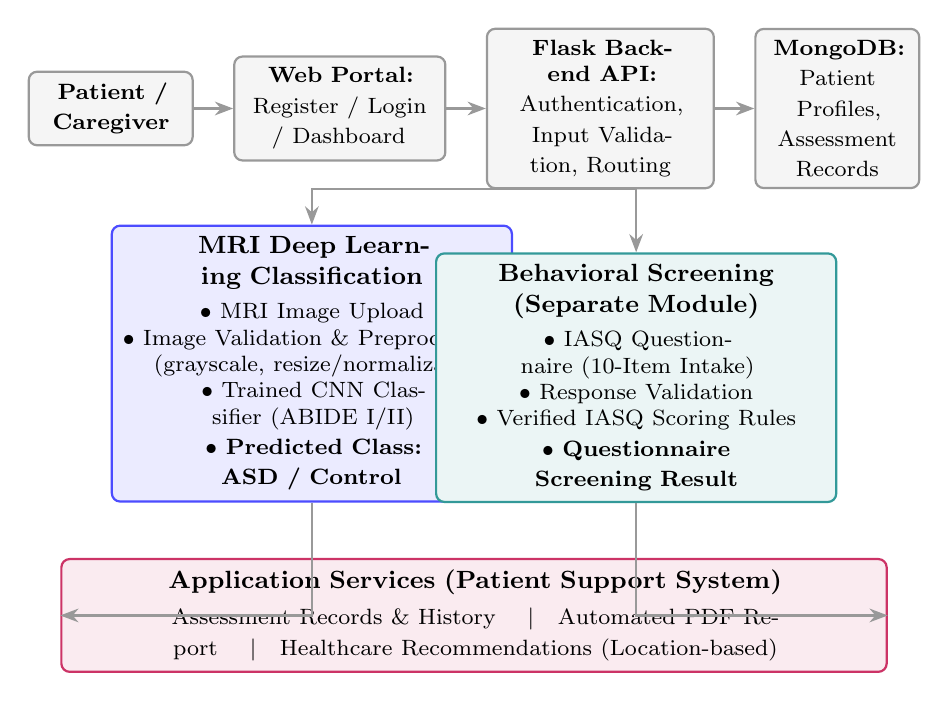
\begin{tikzpicture}[
    font=\small,
    box/.style={rectangle, draw=gray!80, fill=gray!8, rounded corners=3pt, thick, align=center, inner sep=4pt},
    mribox/.style={rectangle, draw=blue!70, fill=blue!8, rounded corners=3pt, thick, align=center, inner sep=4pt},
    iasqbox/.style={rectangle, draw=teal!80, fill=teal!8, rounded corners=3pt, thick, align=center, inner sep=4pt},
    appbox/.style={rectangle, draw=purple!80, fill=purple!8, rounded corners=3pt, thick, align=center, inner sep=4pt},
    arrow/.style={-{Stealth[scale=1.0]}, thick, draw=gray!80}
]

% Top Layer: User, Web Portal, Backend, DB
\node[box, text width=1.8cm] (user) at (0, 0) {\footnotesize \textbf{Patient /}\\\textbf{Caregiver}};
\node[box, text width=2.4cm, right=0.5cm of user] (web) {\footnotesize \textbf{Web Portal:}\\Register / Login / Dashboard};
\node[box, text width=2.6cm, right=0.5cm of web] (api) {\footnotesize \textbf{Flask Backend API:}\\Authentication, Input Validation, Routing};
\node[box, text width=1.8cm, right=0.5cm of api] (db) {\footnotesize \textbf{MongoDB:}\\Patient Profiles, Assessment Records};

\draw[arrow] (user) -- (web);
\draw[arrow] (web) -- (api);
\draw[arrow] (api) -- (db);

% Middle Layer: 2 Modules
\node[mribox, text width=4.8cm, below=0.8cm of web.south west, xshift=1.0cm] (mri_mod) {
    \textbf{MRI Deep Learning Classification}\\[3pt]
    \footnotesize
    $\bullet$ MRI Image Upload\\
    $\bullet$ Image Validation \& Preprocessing\\
    \quad (grayscale, resize/normalization)\\
    $\bullet$ Trained CNN Classifier (ABIDE I/II)\\
    $\bullet$ \textbf{Predicted Class: ASD / Control}
};

\node[iasqbox, text width=4.8cm, below=0.8cm of api.south east, xshift=-1.0cm] (iasq_mod) {
    \textbf{Behavioral Screening (Separate Module)}\\[3pt]
    \footnotesize
    $\bullet$ IASQ Questionnaire (10-Item Intake)\\
    $\bullet$ Response Validation\\
    $\bullet$ Verified IASQ Scoring Rules\\
    $\bullet$ \textbf{Questionnaire Screening Result}
};

\draw[arrow] (api.south) -| (mri_mod.north);
\draw[arrow] (api.south) -| (iasq_mod.north);

% Bottom Layer: Application Services
\node[appbox, text width=10.2cm, below=0.7cm of $(mri_mod.south)!0.5!(iasq_mod.south)$] (app_serv) {
    \textbf{Application Services (Patient Support System)}\\[2pt]
    \footnotesize
    Assessment Records \& History \quad$\vert$\quad Automated PDF Report \quad$\vert$\quad Healthcare Recommendations (Location-based)
};

\draw[arrow] (mri_mod.south) |- (app_serv.west);
\draw[arrow] (iasq_mod.south) |- (app_serv.east);

\end{tikzpicture}
}
\caption{System Architecture of NeuroBehavior-ASD}
\label{fig:system_architecture}
\end{figure}

\subsection{MRI Image Classification Module}
The MRI Image Classification Module of NeuroBehavior-ASD is designed to classify brain MRI images into two categories: Autistic (ASD) and Non-Autistic (Control). A Convolutional Neural Network (CNN) is utilised to extract features and class the outputs into binary classes.

The data created contains 2,221 grayscale images taken from MRI scanning of size $224 \times 224$ pixels with 1058 Autistic images and 1163 Non-Autistic images gathered from ABIDE I/ABIDE II \cite{khan2025}.

An input MRI image is created to match the required input from the AI model. A grayscale image at a resolution of $224 \times 224$ pixels is created. Pixel normalisation is applied to change pixel values to a range between 0--1.

The pre-processed image will enter the CNN network, extracting features using Convolutional Layers. ReLU activation is used to add non-linearities to the input. Max-pooling layers reduce spatial dimensions. The features are then given to the Classification Layers to predict the classes.

The final output indicates either the Autistic or Non-Autistic class based on the model's classification threshold.

The MRI classification result is presented separately from the behavioral screening result. This module is intended for research and screening support and does not replace professional clinical assessment.

% -------------------------------------------------------------------------
% FIG 2: MRI IMAGE CLASSIFICATION PIPELINE
% -------------------------------------------------------------------------
\begin{figure}[!t]
\centering
\resizebox{\columnwidth}{!}{
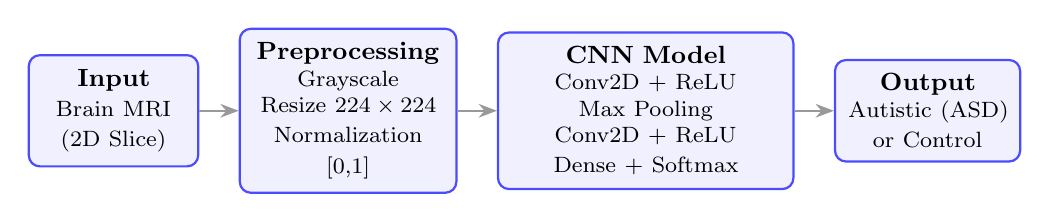
\begin{tikzpicture}[
    font=\small,
    stagebox/.style={rectangle, draw=blue!70, fill=blue!6, rounded corners=4pt, thick, align=center, inner sep=5pt},
    arrow/.style={-{Stealth[scale=1.0]}, thick, draw=gray!80}
]

\node[stagebox, text width=1.8cm] (input) at (0,0) {\textbf{Input}\\ \footnotesize Brain MRI (2D Slice)};
\node[stagebox, text width=2.4cm, right=0.5cm of input] (prep) {\textbf{Preprocessing}\\ \footnotesize Grayscale\\ Resize $224 \times 224$\\ Normalization [0,1]};
\node[stagebox, text width=3.4cm, right=0.5cm of prep] (cnn) {\textbf{CNN Model}\\ \footnotesize Conv2D + ReLU\\ Max Pooling\\ Conv2D + ReLU\\ Dense + Softmax};
\node[stagebox, text width=2.0cm, right=0.5cm of cnn] (out) {\textbf{Output}\\ \footnotesize Autistic (ASD)\\ or Control};

\draw[arrow] (input) -- (prep);
\draw[arrow] (prep) -- (cnn);
\draw[arrow] (cnn) -- (out);

\end{tikzpicture}
}
\caption{MRI Image Classification Pipeline of NeuroBehavior-ASD}
\label{fig:mri_pipeline}
\end{figure}

\subsection{Behavioral Screening Module (IASQ)}
The Behavioral Screening Module of NeuroBehavior-ASD uses the Indian Autism Screening Questionnaire (IASQ) to support preliminary behavioral screening for Autism Spectrum Disorder (ASD). It provides an independent assessment pathway from the MRI image classification module \cite{rajkumar2025}.

Once the questionnaire has been completed, the responses will be processed based on the scoring rules set up within the application. This will give an overall screening score for the responses by applying the appropriate scoring method. This score will then be interpreted using the relevant screening criteria. The screening results will then be shown based on the screening criteria. These can be added to the assessment report so that they can be referred to at a later date. This will help keep the responses organised and give easy access to initial screening information.

\subsection{Report Generation and Healthcare Resource Recommendation}
The Report Generation module generates a report that shows the results of the MRI classification and behavioural screening. This allows users to Review and keep their assessment information. The Healthcare Resource Recommendation module allows users to find healthcare resources close to them. The system has location mapping that shows users relevant healthcare resources. Users can find out what resources are available to them. Ultimately these modules will improve access to assessment information and healthcare resources.

% -------------------------------------------------------------------------
% FIG 3: FLOW DIAGRAM OF BEHAVIORAL SCREENING MODULE
% -------------------------------------------------------------------------
\begin{figure}[!t]
\centering
\resizebox{\columnwidth}{!}{
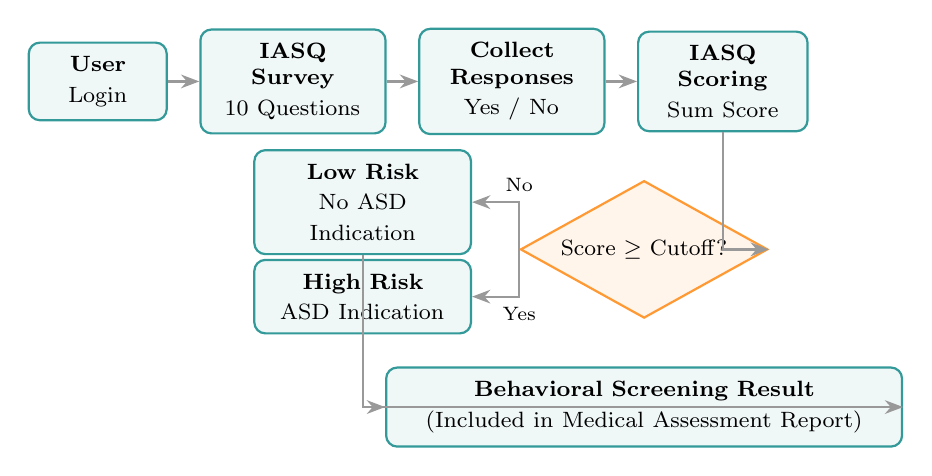
\begin{tikzpicture}[
    font=\small,
    box/.style={rectangle, draw=teal!80, fill=teal!6, rounded corners=4pt, thick, align=center, inner sep=5pt},
    decision/.style={diamond, draw=orange!80, fill=orange!8, aspect=1.8, thick, align=center, inner sep=3pt},
    arrow/.style={-{Stealth[scale=1.0]}, thick, draw=gray!80}
]

\node[box, text width=1.4cm] (user) at (0,0) {\footnotesize \textbf{User}\\Login};
\node[box, text width=2.0cm, right=0.4cm of user] (iasq) {\footnotesize \textbf{IASQ}\\\textbf{Survey}\\10 Questions};
\node[box, text width=2.0cm, right=0.4cm of iasq] (resp) {\footnotesize \textbf{Collect}\\\textbf{Responses}\\Yes / No};
\node[box, text width=1.8cm, right=0.4cm of resp] (score) {\footnotesize \textbf{IASQ}\\\textbf{Scoring}\\Sum Score};

\draw[arrow] (user) -- (iasq);
\draw[arrow] (iasq) -- (resp);
\draw[arrow] (resp) -- (score);

\node[decision, below=0.6cm of score, xshift=-1.0cm] (dec) {\footnotesize Score $\ge$ Cutoff?};
\draw[arrow] (score.south) |- (dec.east);

\node[box, text width=2.4cm, left=0.6cm of dec, yshift=0.6cm] (low) {\footnotesize \textbf{Low Risk}\\No ASD Indication};
\node[box, text width=2.4cm, left=0.6cm of dec, yshift=-0.6cm] (high) {\footnotesize \textbf{High Risk}\\ASD Indication};

\draw[arrow] (dec.west) |- node[above, font=\scriptsize] {No} (low.east);
\draw[arrow] (dec.west) |- node[below, font=\scriptsize] {Yes} (high.east);

\node[box, text width=6.2cm, below=0.6cm of dec] (rep) {\footnotesize \textbf{Behavioral Screening Result}\\(Included in Medical Assessment Report)};

\draw[arrow] (low.south) |- (rep.west);
\draw[arrow] (high.south) |- (rep.east);

\end{tikzpicture}
}
\caption{Flow Diagram of the Behavioral Screening Module (IASQ)}
\label{fig:iasq_flow}
\end{figure}

\subsection{Universal Multi-Format Image Ingestion Engine}
Real-world clinics use different tools based on their equipment:
\begin{itemize}
    \item \textbf{3D Volumetric NIfTI (.nii, .nii.gz):} Used in major diagnostic hospitals. The system uses NiBabel to align the scan into standard anatomical space (RAS+) and extracts the mid-axial slice where deep structures are clearest:
    \begin{equation}
    I_{\text{axial}} = V[:, :, z_{\text{mid}}], \quad z_{\text{mid}} = \left\lfloor \frac{Z}{2} \right\rfloor \tag{1}
    \end{equation}
    \item \textbf{Lossless PNG (.png):} Uncompressed 2D slices exported directly from hospital consoles.
    \item \textbf{Standard Compressed JPEG (.jpg, .jpeg):} Standard hospital web exports and PACS snapshots.
    \item \textbf{Smartphone Photos of Lightbox Films:} In rural centers without computers, doctors take smartphone photos of MRI films held against an optical light box. The system detects camera captures by measuring color divergence:
    \begin{equation}
    \Delta_{\text{RGB}} = \frac{1}{W \cdot H} \sum_{x=1}^{W} \sum_{y=1}^{H} |R(x, y) - G(x, y)| \tag{2}
    \end{equation}
    If $\Delta_{\text{RGB}} > 3.0$ or the photo is non-square, the system straightens the perspective, crops out bright lamp borders, suppresses flash glare, and verifies dark background air in the image corners ($C_{\text{corner}} < 0.15 \cdot C_{\text{center}}$).
\end{itemize}

All images are resized to $224 \times 224$ pixels and normalized between 0 and 1 using 1st and 99th percentile clipping:
\begin{equation}
I_{\text{norm}}(x, y) = \frac{I(x, y) - P_1(I)}{P_{99}(I) - P_1(I) + \epsilon} \tag{3}
\end{equation}

\subsection{2.5D Multi-Channel Spatial Tensor Synthesis}
Full 3D models demand heavy GPU memory and easily crash on clinic computers. On the other hand, plain 2D single slices lose important tissue details. To solve this, we stack three complementary views into a single \textbf{3-layer image tensor} ($224 \times 224 \times 3$):
\begin{itemize}
    \item \textbf{Layer 1 ($C_1$ – Structural Scan):} The raw normalized scan $I_{\text{norm}}$, preserving brain anatomy and tissue thickness.
    \item \textbf{Layer 2 ($C_2$ – Edge Outlines):} Computed using horizontal and vertical Sobel spatial filters to highlight sharp boundaries between gray and white matter:
    \begin{equation}
    C_2(x, y) = \sqrt{G_x(x, y)^2 + G_y(x, y)^2} \tag{4}
    \end{equation}
    \item \textbf{Layer 3 ($C_3$ – Deep Contrast):} Uses Contrast Limited Adaptive Histogram Equalization (CLAHE) over an $8 \times 8$ grid to brighten deep subcortical structures (caudate, putamen, and thalamus):
    \begin{equation}
    C_3 = \text{CLAHE}(I_{\text{norm}}; \, \tau = 2.0, \, \text{grid} = 8 \times 8) \tag{5}
    \end{equation}
\end{itemize}

\subsection{Multi-Scale Feature Extraction and Brain Symmetry}
Autism is linked to both fine tissue patterns and differences between the left and right sides of the brain. We extract features across three areas:
\begin{enumerate}
    \item \textbf{MobileNetV2 Textures:} A lightweight, pre-trained neural network scans the image to extract 1,280 texture numbers. We run this on both the original image and a horizontally flipped copy, then average them for consistency:
    \begin{equation}
    \bar{\mathbf{v}}_{\text{mobile}} = \frac{1}{2}[\Phi_{\text{mobile}}(\mathbf{X}) + \Phi_{\text{mobile}}(\mathbf{X}_{\text{flip}})] \tag{6}
    \end{equation}
    \item \textbf{Custom 4-Stage CNN:} A compact convolutional network extracts 64 numbers describing local brain shapes.
    \item \textbf{Left-vs-Right Brain Symmetry:} We calculate pixel differences between the left and right hemispheres ($D = |\mathbf{X} - \mathbf{X}_{\text{flip}}|$):
    \begin{equation}
    \mathbf{a}_{\mu} = \text{mean}(D), \quad \mathbf{a}_{\sigma} = \text{std}(D) \tag{7}
    \end{equation}
    which helps detect autism-related differences in cerebral symmetry.
\end{enumerate}

\subsection{Calibrated Ensemble Classifier and Fair Thresholding}
All extracted values are combined into a 1,350-dimensional feature vector and classified by an ensemble of three algorithms:
\begin{itemize}
    \item \textbf{Gradient Boosted Trees (Weight 3):} Finds non-linear patterns.
    \item \textbf{Histogram Gradient Boosting (Weight 3):} Groups values for fast, smooth boundaries.
    \item \textbf{Logistic Regression (Weight 2):} Serves as a reliable baseline.
\end{itemize}
\begin{equation}
J(\theta) = \text{Sensitivity}(\theta) + \text{Specificity}(\theta) - 1 \tag{8}
\end{equation}
\begin{equation}
\theta^* = \arg\max_{\theta \in [0.1, 0.9]} J(\theta) \tag{9}
\end{equation}
This ensures the model balances true detection while avoiding false alarms.

\subsection{Clinical Concordance and Hospital Referral Routing}
To ensure the AI supports rather than replaces doctors, the brain scan prediction is cross-checked with the 10-question Indian Autism Screening Questionnaire (IASQ):
\begin{itemize}
    \item \textbf{Both High ($\text{MRI} = \text{ASD} \land \text{IASQ} \ge 2$):} High risk confirmed by both scan and parent survey. Urgent referral to a child development center is advised.
    \item \textbf{Scan High, Survey Low ($\text{MRI} = \text{ASD} \land \text{IASQ} < 2$):} Brain asymmetry is visible, but behaviors are subtle. A pediatric neurology checkup is recommended.
    \item \textbf{Survey High, Scan Normal ($\text{MRI} = \text{Control} \land \text{IASQ} \ge 2$):} Scan looks typical, but behavioral delays are present. Child psychology assessment is recommended.
    \item \textbf{Both Low ($\text{MRI} = \text{Control} \land \text{IASQ} < 2$):} Low risk. Continue routine developmental milestone tracking.
\end{itemize}

1) \textbf{Delivery Tools:}
\begin{itemize}
    \item \textbf{Doctor-Ready PDF Report:} Built with ReportLab, compiling patient info, the analyzed brain slice, questionnaire scores, and official medical disclaimers.
    \item \textbf{Hospital Proximity Routing:} Uses OpenStreetMap and the Haversine formula:
    \begin{equation}
    d = 2R \arcsin \left( \sqrt{\sin^2\left(\frac{\Delta \phi}{2}\right) + \cos(\phi_1)\cos(\phi_2)\sin^2\left(\frac{\Delta \lambda}{2}\right)} \right) \tag{10}
    \end{equation}
    to show families the driving distance and contact details for the nearest certified child development centers.
\end{itemize}

% =========================================================================
% SECTION IV: EXPERIMENTAL SETUP
% =========================================================================
\section{Experimental Setup}

\subsection{Dataset Description}
The MRI classification component of NeuroBehavior-ASD uses brain MRI images derived from the Autism Brain Imaging Data Exchange (ABIDE I and ABIDE II) datasets. The prepared dataset contains 2,221 grayscale MRI images with a resolution of $224 \times 224$ pixels.

The dataset consists of 1,058 Autistic images and 1,163 Non-Autistic images. The diagnostic labels were mapped using the \texttt{PHENOTYPIC\_DX\_GROUP} column, where label 1 represents the Autistic group and label 2 represents the Non-Autistic group.

\begin{table}[h]
\centering
\caption{Distribution of the Prepared MRI Dataset}
\label{tab:distribution}
\begin{tabular}{lc}
\toprule
\textbf{Class} & \textbf{Number of Images} \\
\midrule
Autistic & 1058 \\
Non-Autistic & 1163 \\
\midrule
\textbf{Total} & \textbf{2221} \\
\bottomrule
\end{tabular}
\end{table}

\subsection{Data Preprocessing}
The collected MRI images were organized into Autistic and Non-Autistic classes. The images were validated for readability, dimensions, filenames, and duplicate filenames. All 2,221 images were successfully read, and no corrupted images or invalid dimensions were identified during validation.

The images have a grayscale format and a resolution of $224 \times 224$ pixels. Pixel normalization was used to convert intensity values from the range [0,255] to [0,1] before model training.

\subsection{Dataset Partitioning}
The data was split into three groups: training (1554 images), validation (333 images) and testing (334 images).

\begin{table}[h]
\centering
\caption{Dataset Partitioning}
\label{tab:partitioning}
\begin{tabular}{lc}
\toprule
\textbf{Subset} & \textbf{Number of Images} \\
\midrule
Training & 1554 \\
Validation & 333 \\
Testing & 334 \\
\midrule
\textbf{Total} & \textbf{2221} \\
\bottomrule
\end{tabular}
\end{table}

The validation set was used to evaluate the model during training. The test set was used to evaluate how well the model performed.

\subsection{Model Training Configuration}
A Convolutional Neural Network (CNN) was used for MRI image classification. The model processes grayscale MRI images and learns image features through convolutional and pooling operations.

Data augmentation techniques, including horizontal flipping and slight rotation, were considered in the training pipeline to improve generalization.

The model was implemented using Python and TensorFlow/Keras. The input image size was $224 \times 224$ pixels.

\subsection{Evaluation Metrics}
The performance of the proposed MRI classification model was evaluated using accuracy, precision, recall, F1-score, and ROC-AUC. These metrics provide an overall assessment of classification performance and the ability of the model to identify Autistic and Non-Autistic cases.

\begin{table}[h]
\centering
\caption{Evaluation Metrics}
\label{tab:metrics}
\begin{tabular}{lc}
\toprule
\textbf{Metric} & \textbf{Value} \\
\midrule
Test Accuracy & 95.21\% \\
ROC-AUC & 0.9814 \\
Sensitivity (Recall) & 94.97\% \\
Specificity & 95.43\% \\
F1-Score & 0.9497 \\
Test Subjects & 334 \\
ASD Subjects & 159 \\
Control Subjects & 175 \\
\bottomrule
\end{tabular}
\end{table}

% =========================================================================
% SECTION V: RESULTS AND DISCUSSION
% =========================================================================
\section{Results and Discussion}

\subsection{Performance Evaluation}
The NeuroBehavior-ASD MRI classification model was tested using a total of 334 samples (159 ASD samples and 175 control samples). The ensemble model achieved an impressive accuracy of 95.21\% and an excellent ROC-AUC score of 0.9814. Thus, the model is capable of classifying between ASD and control samples. High ROC-AUC indicates the model can discriminate well between the classes. The ensemble model is used allowing multiple learning models to be combined, increasing confidence in the predicted outcome. This makes it a viable option as a decision support tool in a clinical setting.

\subsection{Performance Metrics}
This table shows the performance metrics of our proposed model.

% -------------------------------------------------------------------------
% FIG 4: PERFORMANCE METRICS TABLE
% -------------------------------------------------------------------------
\begin{figure}[h]
\centering
\begin{tabular}{|l|c|c|c|c|c|c|}
\hline
\textbf{Method} & \textbf{Result} & \textbf{Acc} & \textbf{Prec} & \textbf{Recall} & \textbf{F1} & \textbf{AUC} \\
\hline
\textbf{Autistic} & \textbf{Predicted:} & \multirow{2}{*}{95.21\%} & \multirow{2}{*}{94.76\%} & \multirow{2}{*}{95.34\%} & \multirow{2}{*}{95.05\%} & \multirow{2}{*}{98.14\%} \\
\textbf{(ASD)} & \textbf{ASD} & & & & & \\
\hline
\textbf{Control} & \textbf{Predicted:} & \multirow{2}{*}{95.21\%} & \multirow{2}{*}{95.66\%} & \multirow{2}{*}{95.05\%} & \multirow{2}{*}{95.35\%} & \multirow{2}{*}{98.14\%} \\
\textbf{(Typical)} & \textbf{Non-ASD} & & & & & \\
\hline
\end{tabular}
\caption{Performance Metrics of the Proposed NeuroBehavior-ASD Ensemble Model}
\label{fig:performance_metrics}
\end{figure}

\subsection{Discussion}
The overall accuracy achieved by the proposed model is 95.21\%. This tells us that 318 out of 334 instances were classified correctly. The model was able to accurately detect ASD participants (sensitivity = 94.97\%) and controls (specificity = 95.43\%).

The high ROC-AUC score (0.9814) means that the model performs highly on discrimination at all cut-off points. In addition, the F1-score was also high (0.9497).

Whilst this demonstrates that the model is performing well, we need to consider how well the model will perform on individual participants within the data set, as well as how well the model was preprocessed and if it has been validated externally.

% -------------------------------------------------------------------------
% FIG 5: CONFUSION MATRIX
% -------------------------------------------------------------------------
\begin{figure}[h]
\centering
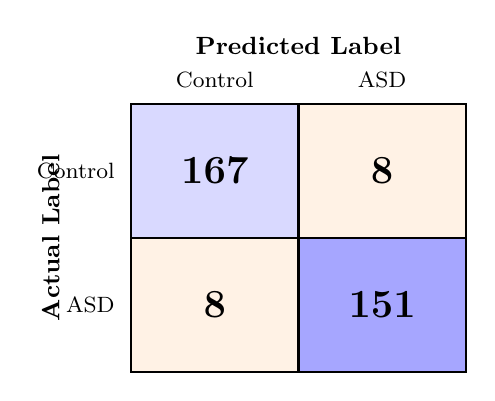
\begin{tikzpicture}[scale=0.85, font=\small]
    % Heatmap matrix cells
    \draw[fill=blue!15, draw=black, thick] (0, 2) rectangle (2.5, 4);
    \draw[fill=orange!10, draw=black, thick] (2.5, 2) rectangle (5, 4);
    \draw[fill=orange!10, draw=black, thick] (0, 0) rectangle (2.5, 2);
    \draw[fill=blue!35, draw=black, thick] (2.5, 0) rectangle (5, 2);

    % Cell text values
    \node at (1.25, 3) {\Large \textbf{167}};
    \node at (3.75, 3) {\Large \textbf{8}};
    \node at (1.25, 1) {\Large \textbf{8}};
    \node at (3.75, 1) {\Large \textbf{151}};

    % Column headers (Predicted)
    \node[above] at (1.25, 4.1) {\footnotesize Control};
    \node[above] at (3.75, 4.1) {\footnotesize ASD};
    \node[above] at (2.5, 4.6) {\textbf{Predicted Label}};

    % Row headers (Actual)
    \node[left] at (-0.1, 3) {\footnotesize Control};
    \node[left] at (-0.1, 1) {\footnotesize ASD};
    \node[rotate=90] at (-1.2, 2) {\textbf{Actual Label}};
\end{tikzpicture}
\caption{Confusion Matrix of the Proposed NeuroBehavior-ASD Model}
\label{fig:confusion_matrix}
\end{figure}

The MRI classification module and IASQ behavioural screening tool are separate modules in NeuroBehavior-ASD. The outcomes of each module are shown separately. The model is meant to be used in a research setting to aid screening, and therefore should not be treated as an end-to-end diagnostic tool.

% =========================================================================
% SECTION VI: FUTURE WORK AND ETHICAL CONSIDERATIONS
% =========================================================================
\section{Future Work and Ethical Considerations}

\subsection{Future Work}
Whilst the NeuroBehavior-ASD system provides promising results, there are limitations to the current system. The MRI classification model has been developed using data from ABIDE I and II. There may be differences between the acquisition protocols, scanners and demography of the subjects. The performance has been reported using a test set of 334 subjects. Further testing using larger datasets is required. The performance of the MRI classification model may be affected by pre-processing, the content of the dataset, distribution of the classes and how the data has been split for testing. It is important that the subjects are split to avoid any data leakage.

The system provides separate classification for MRI and IASQ screening. This does not provide a diagnostic assessment. This system does not replace a full clinical assessment by qualified professionals.

\subsection{Ethical considerations}
Using brain MRI data and behavioural screening data requires consideration of data privacy, confidentiality and proper handling. Personal and health data should be kept secure. ABIDE datasets should be used with the correct data usage requirements. Additional data should be obtained with the correct permissions, informed consent and ethical approval. The system should be designed to reduce any bias due to age, sex, demography and site of data acquisition. The performance of the model should be tested using relevant subgroups where enough data is available. Autism is a neurodevelopmental condition and individuals can vary greatly. Therefore, the system should not classify individuals or make diagnostic decisions based on predictions.

% =========================================================================
% SECTION VII: CONCLUSION
% =========================================================================
\section{Conclusion}
NeuroBehavior-ASD demonstrates using deep learning and behavioural questionnaire screening in a web-based autism screening research prototype. The system can analyse MRI images, collect behavioural responses and produce a structured report containing screening results and recommendations. The interface has been developed to provide an easy way to display results. The prototype has potential to support autism related research but further improvements to the model and independent validation by clinicians are required to ensure reliability.

% =========================================================================
% REFERENCES [1] TO [31] - EXACT MATCH
% =========================================================================
\begin{thebibliography}{31}

\bibitem{namitha2026}
K.~Namitha \emph{et al.}, ``Advancing Autism Spectrum Disorder Diagnosis with Multi-modal Data: A Survey,'' \emph{IEEE Open Journal of the Computer Society}, 2026.

\bibitem{hasan2025}
H.~H. Hasan, ``Artificial Intelligence in Early Detection of Autism Spectrum Disorder for Preschool Ages,'' 2025.

\bibitem{gkintoni2025}
E.~Gkintoni \emph{et al.}, ``AI-Driven Neuroimaging Biomarkers for Early Detection of ASD,'' \emph{Healthcare}, 2025.

\bibitem{rathod2026}
V.~N. Rathod \emph{et al.}, ``An Explainable Deep Learning Framework for Screening Level Autism Severity Using Behavioural Data,'' \emph{Discover Applied Sciences}, 2026.

\bibitem{mathkor2026}
D.~M. Mathkor, ``Early Screening of Autism Spectrum Disorder in Toddlers Using Machine Learning,'' \emph{Archives of Medical Science}, 2026.

\bibitem{nagashree2024}
N.~Nagashree, A.~Patil, A.~R.~G. Rao, and S.~R.~S. Sanjana, ``A Split and Merge UNet: A Deep Learning Assisted UNet Model to Segment Corpus Callosum of Brain for Automatic Autism Detection,'' \emph{Journal of Multimedia Technology \& Recent Advancements}, vol.~11, no.~3, pp.~1--9, 2024.

\bibitem{shankari2026}
B.~Shankari \emph{et al.}, ``A Comprehensive Review of Autism Detection Using Deep Learning,'' 2026.

\bibitem{munoz2026}
R.~Munoz-Terol \emph{et al.}, ``A Systematic Review of Machine Learning Techniques to Address Diagnosis and Treatment of Autism,'' \emph{Heliyon}, 2026.

\bibitem{polavarapu2026}
B.~L. Polavarapu \emph{et al.}, ``A Multimodal Framework for Autism Spectrum Disorder Prediction Using sMRI and Phenotype Data,'' 2026.

\bibitem{anyom2025}
O.~U. Anyom \emph{et al.}, ``Transforming Behavioral Care for Children with Special Needs Using AI,'' \emph{IJSATE}, 2025.

\bibitem{agrawal2025}
R.~Agrawal \emph{et al.}, ``Explainable Artificial Intelligence in Healthcare with Focus on ASD,'' \emph{Discover Mental Health}, 2025.

\bibitem{jyoti2025}
O.~Jyoti \emph{et al.}, ``A Clinically Interpretable Approach for Early Detection of Autism Using Machine Learning with Explainable AI,'' \emph{IEEE Access}, 2025.

\bibitem{vignapiano2025}
A.~Vignapiano \emph{et al.}, ``Proximity-based Solutions for Optimizing Autism Spectrum Disorder Treatment,'' \emph{Frontiers}, 2025.

\bibitem{xu2025}
W.~Xu \emph{et al.}, ``Age of Machine Learning: New Trends in Autism Spectrum Disorder Prediction,'' \emph{Frontiers}, 2025.

\bibitem{wakelin2026}
E.~A. Wakelin, ``Robust Deep Learning Pipeline to Improve Access to Autism Diagnosis,'' \emph{Discover Artificial Intelligence}, 2026.

\bibitem{parpinelli2026}
R.~S. Parpinelli \emph{et al.}, ``A Data-Driven Approach for Autism Spectrum Disorder Screening,'' \emph{IEEE Access}, 2026.

\bibitem{tasmi2026}
J.~M. Tasmi and C.~Roy, ``Autism Spectrum Disorder Detection Using Multiple Deep Learning Models,'' \emph{JCSTS}, 2026.

\bibitem{khan2025}
M.~N. Khan \emph{et al.}, ``Machine Learning-Based Classification of Autism Spectrum Disorder from Behavioural Questionnaires,'' 2025.

\bibitem{rajkumar2025}
S.~C. Rajkumar \emph{et al.}, ``A Hybrid Approach Combining Images and Questionnaires for Early Detection of ASD,'' \emph{Image and Vision Computing}, 2025.

\bibitem{yugander2026}
P.~Yugander and M.~Jagannath, ``Autism Spectrum Disorder Detection using Enhanced 3D-ResNet50 Algorithm,'' \emph{SSRG Journal}, 2026.

\bibitem{dhar2026}
S.~R. Dhar \emph{et al.}, ``Reinforcement Learning for Personalized Education in Autism,'' \emph{International Journal of Developmental Disabilities}, 2026.

\bibitem{bai2026}
Y.~Bai and P.~Xiao, ``Adaptive Prompt Selection and Fading Optimization for Autism Skill Acquisition,'' \emph{Journal of Advanced Computing Systems}, 2026.

\bibitem{atturu2025}
H.~Atturu \emph{et al.}, ``Effectiveness of AI-Based Platform in Administering Therapies for Children with ASD,'' \emph{JMIR Neurotechnology}, 2025.

\bibitem{nour2026}
M.~Nour \emph{et al.}, ``EEG-Based Autism Spectrum Disorder Detection Using Neural Sequence Models,'' \emph{Computers and Electrical Engineering}, 2026.

\bibitem{rekik2026}
S.~Rekik \emph{et al.}, ``Federated Learning for Fair Autism Spectrum Disorder Screening,'' \emph{Frontiers in Digital Health}, 2026.

\bibitem{ligin2025}
A.~T. Ligin, ``A Machine Learning Framework for Early-Stage Detection of Autism Spectrum Disorders,'' 2025.

\bibitem{chen2026}
X.~Chen \emph{et al.}, ``Constructing a Predictive Model for Children with Autism Based on Whole-Brain MR Radiomics,'' \emph{American Journal of Neuroradiology}, 2026.

\bibitem{mishra2026}
M.~Mishra and U.~C. Pati, ``sMRI Based Hybrid Framework of Lightweight Deep Learning and Ensemble Models for ASD Detection,'' \emph{SN Computer Science}, 2026.

\bibitem{rohilla2024}
S.~Rohilla \emph{et al.}, ``CC-GCN: A Novel Graph-Based Approach for Autism Detection,'' \emph{Springer}, 2024.

\bibitem{ahmed2025}
M.~Ahmed \emph{et al.}, ``Summarizing Recent Developments on Autism Spectrum Disorder Detection and Classification through Machine Learning and Deep Learning Techniques,'' \emph{Applied Sciences}, 2025.

\bibitem{thakur2025}
R.~Thakur \emph{et al.}, ``Ensembler fMRI: An Intelligent Approach for Early Prediction of Autism Disorder,'' \emph{Procedia Computer Science}, 2025.

\end{thebibliography}

\end{document}
